\documentclass{article}%
\usepackage[T1]{fontenc}%
\usepackage[utf8]{inputenc}%
\usepackage{lmodern}%
\usepackage{textcomp}%
\usepackage{lastpage}%
\usepackage[head=40pt,margin=0.5in,bottom=0.6in]{geometry}%
\usepackage{graphicx}%
%
\title{\textbf{Cecodap: El Estado abandonó a niños y adolescentes}}%
\author{JOSÉ GREGORIO MEZA}%
\date{05/12/2018}%
%
\begin{document}%
\normalsize%
\maketitle%
\textbf{URL: }%
http://www.el{-}nacional.com/noticias/sociedad/cecodap{-}estado{-}abandono{-}ninos{-}adolescentes\_262149\newline%
%
\textbf{Periodico: }%
EN, %
ID: %
262149, %
Seccion: %
Sociedad\newline%
%
\textbf{Palabras Claves: }%
NO\_TIENE\newline%
%
\textbf{Derecho: }%
5, %
Otros Derechos: %
2.2, %
Sub Derechos: %
2.2.1\newline%
%
\textbf{EP: }%
NO\newline%
\newline%
%
\textbf{\textit{El trabajo resalta que 68,4\% de los programas de protección en el área metropolitana de Caracas se sustenta con recursos privados}}%
\newline%
\newline%
%
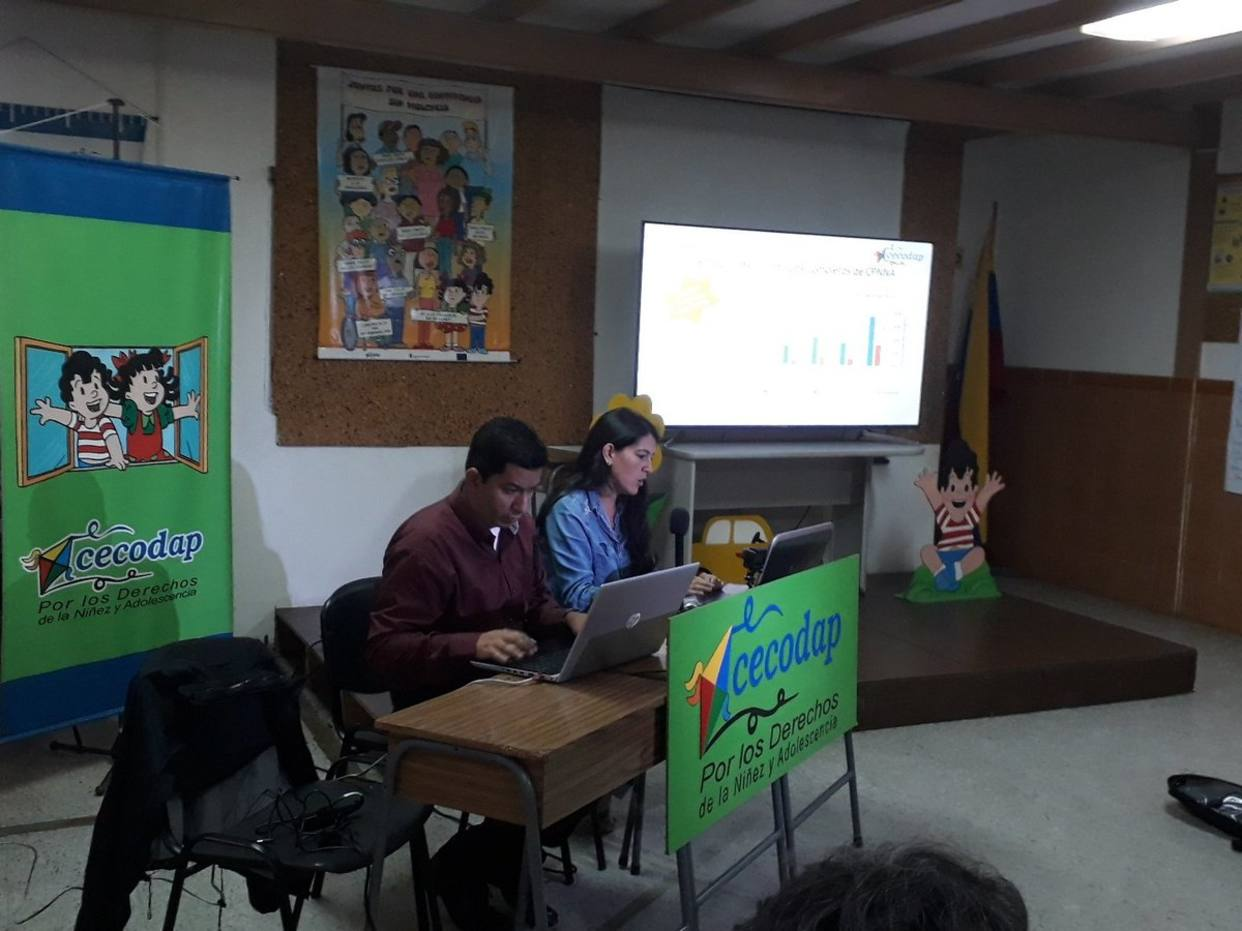
\includegraphics[width=300px]{44.jpg}%
\newline%
%
El Estado ha abandonado la responsabilidad en la atención de niños, niñas y adolescentes, lo que se traduce en una desprotección estructural e institucional, concluyó Cecodap a través de un análisis de las realidades y debilidades del sistema de apoyo en el área metropolitana de Caracas.%
\newline%
%
La investigación “¿Niños desprotegidos?”, coordinada por Angeyeimar Gil y María Victoria Fermín, dejó en evidencia que ha disminuido la capacidad de atención de los consejos de protección debido a las fallas operativas y no a la disminución de casos de violencia contra niños.%
\newline%
%
El trabajo resalta que 68,4\% de los programas se sustenta con recursos privados.%
\newline%
%
Solo en Baruta se han reportado 500 niños en situación de calle. En El Hatillo hay 147 y en Chacao 44.%
\newline%
%
Gil informó que en el proceso de recolección de información no tuvieron acceso a fuentes oficiales en Libertador. En los otros municipios sí cooperaron con entrevistas y datos.%
\newline%
%
Dijo que en el área metropolitana de Caracas ningún ente municipal posee la cantidad de consejeros necesarios para poder garantizar el apoyo adecuado. “La niñez y la adolescencia en Venezuela se han convertido en una población con mayor vulnerabilidad en comparación con los niños, niñas y adolescentes en otros países, resultado de la situación de emergencia humanitaria compleja que vivimos”, resaltó.%
\newline%
%
Explicó que la migración del país es la razón principal que aducen los consejeros para renunciar a sus cargos. La alta rotación incide en la pérdida de personal capacitado.%
\newline%
%
La investigación detalla que los bajos sueldos que se ofrecen en las alcaldías para posiciones de tal responsabilidad social dificultan que nuevos profesionales entren y ayuden a estabilizar el servicio.%
\newline%
%
“Nos preocupa que se observa un cierre técnico de los consejos. Hay más de 57\% de ausencia en los equipos”, indicó.%
\newline%
%
“Los programas de atención son la base del sistema de apoyo previsto por la Lopna. La ausencia de planes que la investigación observó evidencia la falta de capacidad de respuesta”, afirmó Fernando Pereira, educador y fundador de Cecodap.%
\newline%
%
Señaló que el Estado está ausente: no dicta políticas acordes con la realidad, no aporta presupuesto, no cuenta con un sistema de información y monitoreo sobre la realidad de los niños y adolescentes.%
\newline%
%
Aseveró que es imposible que se puedan garantizar efectivamente los derechos humanos de esta población vulnerable solo con el trabajo voluntario, la cooperación de la sociedad civil y con el exiguo presupuesto público.%
\newline%
%
“La crisis en el sistema de protección en términos de recursos humanos y materiales conduce a incumplir los protocolos de atención, víctimas de la vulneración de sus derechos”, indicó Carlos Trapani, abogado y coordinador general de Cecodap.%
\newline%
%
\end{document}